\section{Theorie}
\label{sec:theorie}

In allen Atomen befinden sich Elektronen auf sogenannten Schalen um den
Atomkern. Auf diesen Schalen besitzen sie feste Energien, zwischen welchen
allerdings Übergänge stattfinden können. Dazu muss Energie, die exakt der
Differenz der Niveaus entspricht von den Elektronen abgegeben oder aufgenommen
werden. Dies geschieht über die Aufnahme oder Abgabe von Photonen der
passenenden Frequenz. Die äußeren Niveaus, also jene mit den größten Energien,
sind dabei je nach Temperatur unterschiedlich besetzt. Die Besetzungszahl eines
Niveaus ist dabei Boltzmann-verteilt, sodass für das Verhältnis der
Besetzungszahlen zweier Niveaus gilt:
%
\begin{equation}
  \frac{N_2}{N_1}=\frac{\symup{g_2}}{\symup{g_1}}\frac{e^{-\sfrac{W_2}{\symup{k_B}T}}}{e^{-\sfrac{W_1}{\symup{k_B}T}}}
\end{equation}
%
Hierbei beschreiben die $W_i$ die Energien der Zustände, die $\symup{g_i}$ die
Lande-Faktoren, welche beschrieben wieviele Zustände zu der entsprechenden
Energie gehören, sowie $\symup{k_B}$ die Boltzmann-Konstante und $T$ die
Temperatur. \\
Mit Hilfe des optischen Pumpens kann eine Abweichung von dieser Verteilung
erzeugt werden. Diese kann soweit gehen, dass eine Besetzungsinversion
entsteht. Eine so entstehende nicht-thermische Verteilung ermöglicht es,
einzelne Übergänge zu induzieren, sodass Photonen dieser Energie überwiegend
das Spektrum prägen. Über die Vermessung dieses Lichtes lässt sich der
Energieabstand $\symup{h}\nu=W_2-W_1$ der Niveaus messen.

\subsection{Energieniveaus der Elektronen eines Atomes}
%
Die Verteilung der Elektronen auf verschiedene Energieniveaus innerhalb des
Atomes folgt aus Auswahlregeln verschiedener Quantenzahlen. Aus dem
Gesamtdrehimpuls $\vec{J}$ der Elektronenhülle folgt ein magnetisches Moment
$\vec{\mu}_J=-\symup{g_J}\symup{\mu_B}\vec{J}$. Der Faktor $\symup{g_J}$
berücksichtigt dabei, dass das Gesamtmoment aus Spin $S$ und Drehimpuls $L$
folgt. Es gilt
%
\begin{align*}
  |\vec{\mu_J}|=&\symup{g_J}\symup{\mu_B}\sqrt{J(J+1)}, \;\text{wobei} \\
  |\vec{\mu_L}|=&-\symup{\mu_B}\sqrt{L(L+1)} \;\text{und} \\
  |\vec{\mu_S}|=&-\symup{g_S}\symup{\mu_B}\sqrt{S(S+1)} \, .
\end{align*}
%
Das Gesamtdrehmoment $\vec{\mu_J}$ der Elektronenhülle präzediert dabei um den
Gesamtdrehimpuls $\vec{J}$. Daher trägt stets nur der parallele Anteil dieses
Drehimpulses zum magnetischen Moment bei. $\symup{g_J}$ ist also abhängig von
$J$, $S$ und $L$. Wird ein äußeres Magnetfeld angelegt, so spaltet sich das
Spektrum weiter auf. Es gilt
%
\begin{equation}
  U_\text{mag}=-\vec{\mu_J}\cdot\vec{B}
\end{equation}
%
Hieraus folgt eine Richtungsquantelung der Energie:
%
\begin{equation}
  U_\text{mag}=\symup{g_J}\symup{\mu_B}B\cdot M_J\, ,\quad M_J\in[-J,J]
\end{equation}
%
Bei Anlegen eines äußeren Magnetfeldes wird also über den Zeeman-Effekt jedes
Energieniveau in $2J+1$ Unterniveaus aufgespalten. Die Anzahl der so
entstehenden Niveaus ist abhängig von der sich aus Gesamtdrehimpuls der
Elektronenhülle $J$ und dem Kernspin $I$ ergebene Gesamtdrehimpuls $F$ des
Atomes.
%
\begin{figure}[htb]
  \centering
  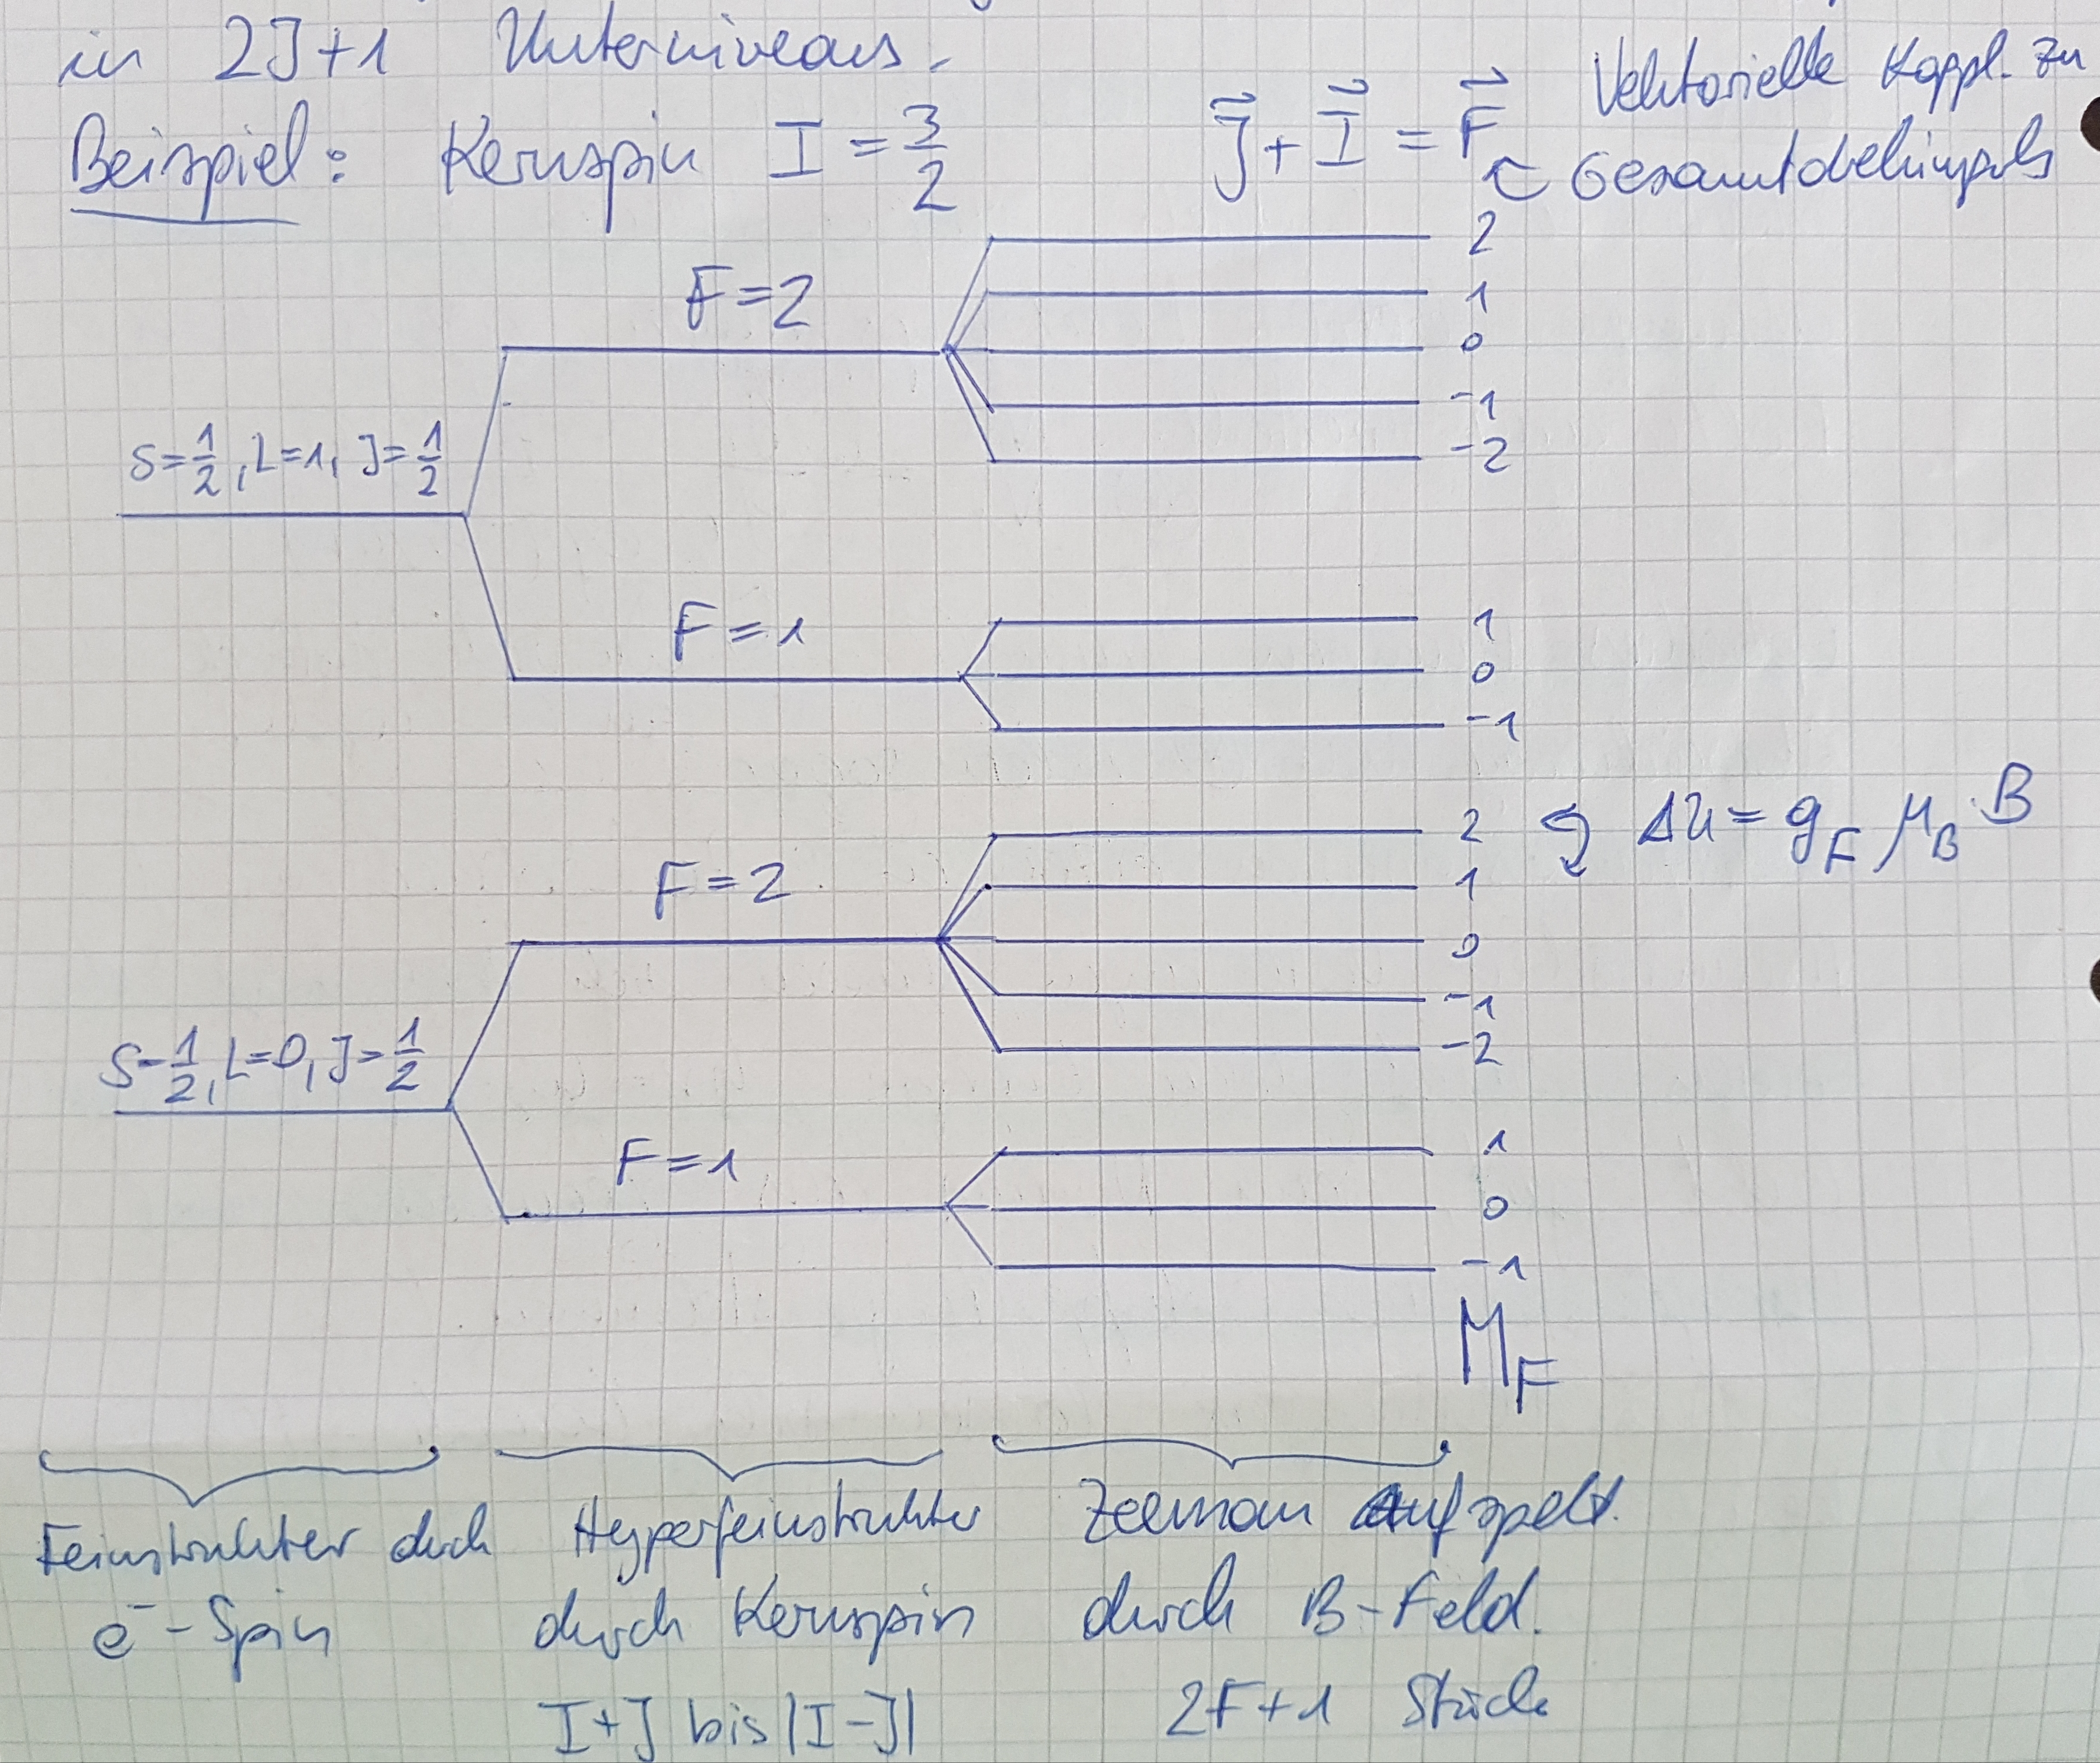
\includegraphics[width=0.75\textwidth]{figures/Aufspaltung.jpg}
  \caption{Aufspaltung der Energieniveaus innerhalb eines Atomes. Dargestellt sind die Feinstrukturaufspaltung durch den Elektronenspin, die Hyperfeinstrukturaufspaltung durch den Kernspin, sowie die Zeeman-Aufspaltung durch ein äußeres Magnetfeld.}
  \label{fig:aufspaltung}
\end{figure}
%
\subsection{Optisches Pumpen}
%
Zum Verständnis des Verfahrens des optischen Pumpens wird ein Beispiel-System
betrachtet. Es handelt sich dabei um ein Atom ohne Kernspin $\vec{I}$. Der
Grundzustand ist der Zustand $^2S_{\sfrac{1}{2}}$. Angeregte Zustände sind
$^2P_{\sfrac{1}{2}}$, sowie $^2P_{\sfrac{3}{2}}$.
%
\begin{figure}[htb]
  \centering
  \includegraphics[width=0.9\textwidth]{figures/Beispiel.jpg}
  \caption{Aufspaltung der $S$- und $P$-Niveaus eines Beispiel-Atomes. Rechts: Zeeman-Aufspaltung des $^2P_{\sfrac{1}{2}}$- sowie des $^2S_{\sfrac{1}{2}}$-Niveaus.}
  \label{fig:beispiel}
\end{figure}
%
Die Energieniveaus, sowie deren Aufspaltung im Magnetfeld sind in
Abbildung~\ref{fig:beispiel} skizziert. Das bei den rechts skizzierten
Übergängen emittierte Licht besitzt spezielle Polarisationseigenschaften. Das
$\sigma^+$-Licht ist rechtszirkular polarisiert (also
$\vec{s}\nparallel\vec{k}$), während das $\sigma^-$-Licht linkszirkular
polarisiert ist (also $\vec{s}\parallel\vec{k}$). Beide Linien erscheinen nur
parallel zum Magnetfeld in dieser Polarisation und sonst linear polarisiert.
Die $\pi$-Linien hingegen sind linear polarisiert und werden nicht parallel zum
Magnetfeld abgestrahlt, da es sich hierbei um Dipolstrahlung handelt.\\
%
\begin{figure}[htb]
  \centering
  \includegraphics[width=\textwidth]{figures/Versuchsaufbau.pdf}
  \caption{Schematische Darstellung des Versuchsaufbaus \cite{V21}.}
  \label{fig:aufbau}
\end{figure}
%
Abbildung~\ref{fig:aufbau} zeigt den schematischen Aufbau der verwendeten
Apperatur. Eine Spektrallampe strahlt Licht in die Apperatur ein. Aus diesem
Licht wird mit Hilfe eines $\text{D}_1$-Filters und eines Polarisationsfilters
rechtszirkular polarisiertes $\text{D}_1$-Licht. Der einzige mögliche
Energieübergang innerhalb der Atome in der Dampfzelle ist derjenige von
$^2\symup{S}_{\sfrac{1}{2}}$ (mit $\symup{M_J}=-\sfrac{1}{2}$) zu
$^2P_{\sfrac{1}{2}}$ (mit $\symup{M_J}=+\sfrac{1}{2}$), sowie rückwärts durch
spontane Emission. Beim rückwärtigen Prozess werden allerdings beide
Zeeman-Niveaus des $^2\symup{S}_{\sfrac{1}{2}}$-Niveaus besetzt, sodass im
Laufe der Zeit das Niveau $^2\symup{S}_{\sfrac{1}{2}}$ (mit
$\symup{M_J}=+\sfrac{1}{2}$) angereichert und das
$^2\symup{S}_{\sfrac{1}{2}}$-Niveau (mit $\symup{M_J}=-\sfrac{1}{2}$)
"leergepumpt" wird. Dies hat eine Umkehr der Bestzung im S-Niveau zur Folge.
Experimentell beobachten lässt sich diese Entwicklung über die Transparenz des
Dampfes für Licht. \\
Wird Licht (einer bestimmten Energie) von dem Dampf absorbiert, so heißt dies,
dass Elektronen im Gas angeregt werden und dabei die Photonen absorbieren. Dies
ist natürlich nur möglich, wenn sich Elektronen in dem unteren Energieniveau
dieser Anregungen befinden. Je weniger Elektronen sich in diesem Niveau
befinden, desto unwahrscheinlicher ist eine Absorbtion des Photons und desto
transparenter erscheint das Gas.\\
Es treten zwei Prozesse zur Abregung, also zur Emission von Photonen aus den
Gesatomen auf. Bei der \textbf{spontanen Emission} begibt sich ein Elektron auf
ein niedrigeres Energieniveau und gibt dabei ein Photon der Energiedifferenz
ab. Bei der \textbf{induzierten Emission} verursacht ein eingestrahltes Photon
den beschriebenen Prozess, sodass hierbei zwei Photonen emittiert werden. Diese
gleichen sich in Energie, Polarisation und Impulsvektor. Welcher dieser beiden
Prozesse überwiegt, hängt von der Energie der Photonen ab. Die
Übergangswahrscheinlichkeit für spontane Emission ist proportional zu $\nu^3$,
und damit bei großen Frequenzen aussschlaggebend. Bei kleineren Energien, wie
etwa denen bei Zeeman-Übergängen kommt es quasi nur zu induzierter Emission.
Dies kann also sehr gut zur Vermessung dieser Übergänge verwendet werden. \\
Die Energiedifferenzen zwischen den Zeeman-Niveaus ist abhängig von der Stärke
des angelegten Magnetfeldes:
%
\begin{equation}
  h\nu=g_{\symup{J}}\mu_{\symup{B}}B\symup{\Delta}M_{\symup{J}} \, .
  \label{eq:übergangsenergie}
\end{equation}
%
Durch Einschalten des Magnetfeldes und Entstehen der Zeeman-Aufspaltung beginnt das oben
beschriebene Pumpen durch spontane Emission bis eine Besetzungsumkehrung eintritt. Wenn
allerdings das Magnetfeld den Wert
%
\begin{equation}
  B_m=\frac{4\pi m_0}{e_0g_J}\nu
\end{equation}
%
annimmt setzt induzierte Emission ein, sodass die Besetzungsinversion wieder
zerfällt. Die Transparenz wird also nachdem sie der 1 zustrebte plötzlich 
wieder kleiner, wenn der oben beschriebene Wert erreicht wird.

\begin{equation}
  g_{\symup{J}}=\frac{\num{3.0023}J(J+1)+\num{1.0023}\left(S(S+1)-L(L+1)\right)}{2J(J+1)}
  \label{eq:gj}
\end{equation}

\begin{equation}
  U_{\symup{HF}}=g_{\symup{F}}\mu_{\symup{B}}B
  +g_{\symup{F}}^2\mu_{\symup{B}}^2B^2
  \frac{(1-2M_{\symup{F}})}{\symup{\Delta}E_{\symup{Hy}}}-\ldots
  \label{eq:zeemanenergie}
\end{equation}
